

\documentclass[12pt,aspectratio=169]{beamer}

% Packages
\usepackage{mathtools}
\usepackage{hyperref}
\usepackage{setspace}
\usepackage{tikz}
\usetikzlibrary{positioning}
\usepackage{ragged2e}
\usepackage{nicematrix}
\usepackage[compatibility=false]{caption}
\usepackage[framemethod=tikz]{mdframed}

% Colored boxes
\usepackage{tcolorbox}
\tcbsetforeverylayer{autoparskip} % Removes unwanted vertical space

% Theme
\usetheme{metropolis}
\metroset{subsectionpage=progressbar,sectionpage=none}
\setbeamertemplate{theorems}[numbered]

\usepackage{fontspec}
\defaultfontfeatures{LetterSpace=30}


% Code
\usepackage{listings}
% Custom colors
\definecolor{codegreen}{rgb}{0,0.6,0}
\definecolor{codegray}{rgb}{0.5,0.5,0.5}
\definecolor{codepurple}{rgb}{0.58,0,0.82}
\definecolor{backcolour}{rgb}{0.95,0.95,0.92}
\definecolor{light-gray}{gray}{0.95}
% Python style for highlighting
\newcommand\pythonstyle{\lstset{
		backgroundcolor=\color{white},
		language=Python,
		basicstyle=\ttfamily\footnotesize,
		morekeywords={self},              % Add keywords here
		keywordstyle=\color{blue},
		stringstyle=\footnotesize\color{deepgreen},
		commentstyle=\color{codegreen},
		showstringspaces=false,
		frame=tb,
		numbers=left,
		numbersep=5pt,
		numberstyle=\tiny\color{gray},
		columns=fullflexible,
		numbersep=5pt,
		aboveskip=1em,
		showtabs=false,
		tabsize=2,
		gobble=3
	}}

% Python environment
\lstnewenvironment{python}[1][]
{
	\pythonstyle
	\lstset{#1}
}
{}
% Python for inline
\newcommand\pythoninline[1]{{\pythonstyle\lstinline!#1!}}

% Tables and justification
\newcommand{\ra}[1]{\renewcommand{\arraystretch}{#1}}
\justifying

% Subfigures
\setbeamertemplate{caption}[numbered]
\usepackage[caption=false,font=footnotesize]{subfig}

% Colors
\setbeamercolor{uppercolgreen}{fg=white,bg=green!35}
\setbeamercolor{lowercolgreen}{fg=black,bg=green!10}
\setbeamercolor{uppercolred}{fg=white,bg=red!35}
\setbeamercolor{lowercolred}{fg=black,bg=red!10}
\setbeamercolor{uppercolblue}{fg=white,bg=blue!35}
\setbeamercolor{lowercolblue}{fg=black,bg=blue!10}
\definecolor{darkred}{rgb}{0.55, 0.0, 0.0}
\definecolor{darkpastelblue}{rgb}{0.47, 0.62, 0.8}
\definecolor{darkcerulean}{rgb}{0.03, 0.27, 0.49}
\definecolor{darkgreen}{rgb}{0.0, 0.55, 0.0}
\definecolor{deepblue}{rgb}{0,0,0.5}
\definecolor{deepred}{rgb}{0.6,0,0}
\definecolor{deepgreen}{rgb}{0,0.5,0}

% Matrix size
\usepackage{stackengine}
\stackMath
\def\sss{\scriptstyle \color{gray}}
\setstackgap{L}{12pt}
\def\stacktype{L}

% Mathematical commands
\newcommand{\vc}[1]{\boldsymbol{\mathbf{#1}}}
\newcommand{\pr}[1]{{#1\,}'}
\newcommand{\idx}[2]{{\color{darkpastelblue}[}#1{\color{darkpastelblue}]_{#2}}}
\newcommand{\shape}[2]{\stackunder{#1}{\sss #2}}
\DeclareMathOperator*{\argmax}{arg\,max}
\DeclareMathOperator*{\argmin}{arg\,min}

% Style commands
\newcommand{\myalert}[1]{{\color{darkred}\textbf{#1}}}

% White frame (for images)
\newenvironment{whiteframe}[1]{
	\setbeamercolor{background canvas}{bg=white}
	\begin{frame}{#1}
		}{
	\end{frame}
}

\setbeamerfont{frametitle}{size=\normalsize}
\setbeamertemplate{frametitle}[default][right]
{
}
%\setbeamercolor{frametitle}{fg=white,bg=black!75}

% No headline frame
\makeatletter
\newenvironment{noheadline}{
	\setbeamertemplate{headline}{}
	\addtobeamertemplate{frametitle}{\vspace*{-3.5\baselineskip}}{}
}{}
\makeatother

% Lists
\setbeamertemplate{itemize items}[triangle]

% Footnotes
\setbeamertemplate{footnote}%
{%
	\parindent 1.5em\noindent%
	\justifying\setstretch{0.7}%
	\hbox to 1em{\hfil\insertfootnotemark}\begin{scriptsize}\insertfootnotetext\end{scriptsize}\par%
}

% Footnote without number
\newcommand\blfootnote[1]{%
	\begingroup
	\renewcommand\thefootnote{}\footnote[frame]{\noindent#1}%
	\addtocounter{footnote}{-1}%
	\endgroup
}

% Theorems
\newcommand*{\theorembreak}{\usebeamertemplate{theorem end}\framebreak\usebeamertemplate{theorem begin}}
\newcounter{theo}[section]\setcounter{theo}{0}
\renewcommand{\thetheo}{\arabic{section}.\arabic{theo}}

\newenvironment{theo}[2][]{%
	\refstepcounter{theo}%
	\ifstrempty{#1}%
	{\mdfsetup{%
			frametitle={%
					\tikz[baseline=(current bounding box.east),outer sep=0pt]
					\node[anchor=east,rectangle,fill=red!10]
					{\strut Theorem~\thetheo};}}
	}%
	{\mdfsetup{%
			frametitle={%
					\tikz[baseline=(current bounding box.east),outer sep=0pt]
					\node[anchor=east,rectangle,fill=red!10]
					{\strut Theorem~\thetheo:~#1};}}%
	}%
	\mdfsetup{innertopmargin=5pt,linecolor=red!10,%
		linewidth=2pt,topline=true,%
		frametitleaboveskip=\dimexpr-\ht\strutbox\relax
	}
	\begin{mdframed}[]\relax%
		\label{#2}}{\end{mdframed}}

% The 2024 source used annotate-equations for optional visual labels.
% Keep the deck portable when that package is unavailable.
\newcommand{\eqnmarkbox}[3][]{#3}
\newcommand{\annotate}[4][]{}
\usepackage{subfig}

% Colors
\definecolor{titlecolor}{RGB}{245, 242, 238} 
\definecolor{drawgray}{HTML}{666666}
\definecolor{drawgray_l}{HTML}{F5F5F5}
\definecolor{drawblue}{HTML}{6C8EBF}
\definecolor{drawblue_l}{HTML}{DAE8FC}
\definecolor{drawgreen}{HTML}{82B366}
\definecolor{drawgreen_l}{HTML}{D5E8D4}
\definecolor{draworange}{HTML}{D79B00}
\definecolor{draworange_l}{HTML}{FFE6CC}
\definecolor{drawyellow}{HTML}{D6B656}
\definecolor{drawyellow_l}{HTML}{FFF2CC}
\definecolor{drawred}{HTML}{B85450}
\definecolor{drawred_l}{HTML}{EA6B66}
\definecolor{drawviolet}{HTML}{9673A6}
\definecolor{drawviolet_l}{HTML}{E1D5E7}

\tcbset{
	nndsblue/.style={colback=drawblue_l!35!white,colframe=drawblue,boxrule=0.8pt,arc=1mm},
	nndsgreen/.style={colback=drawgreen_l!35!white,colframe=drawgreen,boxrule=0.8pt,arc=1mm},
	nndsorange/.style={colback=draworange_l!35!white,colframe=draworange,boxrule=0.8pt,arc=1mm},
	nndsred/.style={colback=drawred_l!12!white,colframe=drawred,boxrule=0.8pt,arc=1mm}
}


\begin{document}

{\usebackgroundtemplate{\tikz\node[opacity=0.4,inner sep=0]{
\includegraphics[width=\paperwidth,height=\paperheight]{images/header}};}%
\begin{frame}[plain]
	\vspace{0.5cm}
	\title{\large \begin{spacing}{1.0}Neural Networks for Data Science\end{spacing}\vspace{0.25em}
		\normalsize \begin{spacing}{1.0}\textbf{Master's Degree in Data Science}\end{spacing}\vspace{0.5em}}
	\subtitle{\Large \textbf{Lecture 4: Fully-connected neural networks}}
	\date{
		{
\includegraphics[scale=0.8]{images/Uniroma1}}
	}
	\author{
		\setlength{\tabcolsep}{2pt}
		\begin{tabular}{rl}
			\textbf{Lecturer}: & S. Scardapane \\
		\end{tabular}
	}\titlepage
\end{frame}
}

\section{Feedforward neural networks}
\subsection{Basic definitions}

\begin{frame}{Linear models are limited}
	\begin{columns}[c,onlytextwidth]
		\begin{column}{0.57\textwidth}
			For binary classification, a linear model separates the two classes using:
			\[
				{\color{darkcerulean}\vc{w}^{\top}\vc{x}+b=0}\,.
			\]
			Such a \myalert{linear boundary} can only separate relatively simple datasets.

			\vspace{0.8em}
			Can we \myalert{learn a representation} of the data where a linear model is sufficient?
		\end{column}
		\begin{column}{0.39\textwidth}
			\centering
			\begin{tikzpicture}[scale=0.95]
				\draw[->,gray] (-1.7,0)--(1.8,0) node[right] {$x_1$};
				\draw[->,gray] (0,-1.7)--(0,1.8) node[above] {$x_2$};
				\draw[dashed,gray,thick] (-1.6,1.15)--(1.6,-0.45);
				\foreach \x/\y in {-1/1,1/-1}{\fill[darkcerulean] (\x,\y) circle (0.10);}
				\foreach \x/\y in {1/1,-1/-1}{\draw[darkred,very thick] (\x-0.09,\y-0.09)--(\x+0.09,\y+0.09);\draw[darkred,very thick] (\x-0.09,\y+0.09)--(\x+0.09,\y-0.09);}
			\end{tikzpicture}

			\small A simple non-linearly separable dataset (XOR).
		\end{column}
	\end{columns}
\end{frame}

\begin{frame}{The multilayer perceptron}
	\setlength{\abovedisplayskip}{5pt}\setlength{\belowdisplayskip}{5pt}
	A \textbf{fully-connected neural network}, also known as a \textbf{multilayer perceptron (MLP)}, learns an intermediate representation of the input:

	\vspace{0.2em}
	\begin{columns}[T,onlytextwidth]
		\begin{column}{0.49\textwidth}
			\begin{tcolorbox}[nndsblue,height=0.42\textheight]
				\textbf{\color{darkcerulean}Hidden representation}
				\[
					{\color{darkcerulean}\vc{h}} = \phi(\vc{W}\vc{x}+\vc{b})
				\]
				\small $\phi$ is an elementwise \textbf{activation function}.
			\end{tcolorbox}
		\end{column}
		\begin{column}{0.49\textwidth}
			\begin{tcolorbox}[nndsgreen,height=0.42\textheight]
				\textbf{\color{darkgreen}Linear output}
				\[
					{\color{darkgreen}f(\vc{x})} = \vc{w}^{\top}{\color{darkcerulean}\vc{h}}+c
				\]
				\small A linear model applied to the learned features $\vc{h}$.
			\end{tcolorbox}
		\end{column}
	\end{columns}

	\vspace{0.5em}
	The parameters $\vc{W},\vc{b},\vc{w},c$ are learned jointly from the data.

	\vfill
	{\scriptsize\color{drawgray}Without the nonlinearity ($\phi(z)=z$), the two affine maps collapse:
		\[
			f(\vc{x})=\vc{w}^{\top}(\vc{W}\vc{x}+\vc{b})+c
			=(\vc{w}^{\top}\vc{W})\vc{x}+(\vc{w}^{\top}\vc{b}+c).
		\]}
\end{frame}

\begin{frame}{Embedding the data}
	\begin{columns}[c,onlytextwidth]
		\begin{column}{0.36\textwidth}
			The hidden representation provides new coordinates for the input, in which a linear output layer can distinguish the classes.
		\end{column}
		\begin{column}{0.60\textwidth}
			\centering
			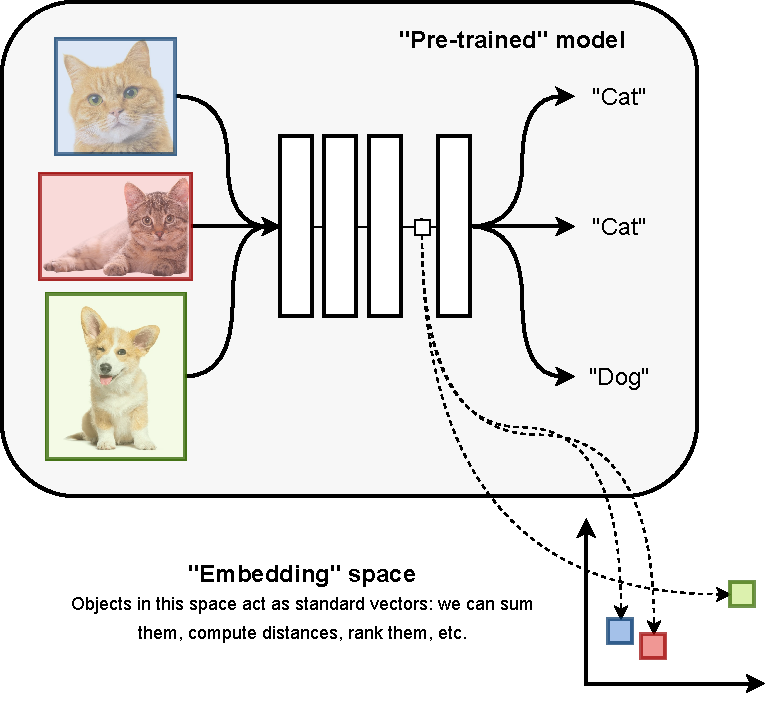
\includegraphics[height=0.80\textheight]{images/lecture_3/embedding.pdf}
		\end{column}
	\end{columns}
\end{frame}

\begin{frame}{Adding hidden layers}
	\small
	\setlength{\jot}{1pt}
	\setlength{\abovedisplayskip}{5pt}\setlength{\belowdisplayskip}{5pt}
	Nothing prevents us from adding additional \textbf{hidden} (intermediate) layers:
	\begin{align*}
		\vc{h}^{(0)}                                       & = \vc{x},                                                                                           \\
		{\color{darkcerulean}\vc{h}^{(\ell)}}              & = \phi_{\ell}\!\left(\vc{W}^{(\ell)}\vc{h}^{(\ell-1)}+\vc{b}^{(\ell)}\right),\quad \ell=1,\ldots,L, \\
		{\color{darkgreen}f_{\boldsymbol{\theta}}(\vc{x})} & = \vc{w}^{\top}\vc{h}^{(L)}+c.
	\end{align*}
	All weights and biases belong to $\boldsymbol{\theta}=\{\vc{W}^{(\ell)},\vc{b}^{(\ell)}\}_{\ell=1}^{L}\cup\{\vc{w},c\}$.

	\medskip
	For widths $D_0,\ldots,D_L$ ($D_0$ is the input dimension),
	\[
		\vc{W}^{(\ell)}\in\mathbb{R}^{D_\ell\times D_{\ell-1}},
		\qquad \vc{b}^{(\ell)}\in\mathbb{R}^{D_\ell}.
	\]
	Layer $\ell$ has $D_\ell(D_{\ell-1}+1)$ parameters; the scalar output adds $D_L+1$.

	\smallskip
	Widths and activations are layer-specific \textbf{hyperparameters}.

\end{frame}

\begin{frame}{Training the network}
	\small
	\setlength{\abovedisplayskip}{6pt}\setlength{\belowdisplayskip}{6pt}
	\begin{tcolorbox}[nndsgreen]
		Given a dataset $\mathcal{S}=\{(\vc{x}_i,y_i)\}_{i=1}^{N}$, we minimize:
		\[
			\boldsymbol{\theta}^{*}=\arg\min_{\boldsymbol{\theta}}\frac{1}{N}\sum_{i=1}^{N}
			\ell\!\left(f_{\boldsymbol{\theta}}(\vc{x}_i),y_i\right).
		\]
	\end{tcolorbox}
	We use the losses introduced in Lecture 3, with the appropriate output for regression or classification (i.e., adding a softmax or sigmoid for multi-class or binary classification, respectively). In order to compute gradients we can use \myalert{automatic differentiation}.
\end{frame}

\begin{frame}{Universal approximation}
	\setlength{\abovedisplayskip}{6pt}\setlength{\belowdisplayskip}{6pt}
	\begin{tcolorbox}[nndsblue]
		\small
		Let $g:K\to\mathbb{R}$ be continuous on a compact set $K\subset\mathbb{R}^{d}$, and let $\phi$ be continuous and non-polynomial.

		For any $\varepsilon>0$, there exists an MLP with \textbf{one hidden layer}, sufficiently large width, and biases such that:
		\[
			\sup_{\vc{x}\in K}\left|g(\vc{x})-f_{\boldsymbol{\theta}}(\vc{x})\right|<\varepsilon.
		\]
	\end{tcolorbox}
	\small
	This is an \textbf{existence result}. It does not tell us how much width or data we need, or whether training will find suitable parameters.

	A single hidden layer can be sufficient for approximation; it need not be an efficient choice.
	\vfill
	{\scriptsize\color{drawgray}Leshno, Lin, Pinkus and Schocken (1993), \href{https://doi.org/10.1016/S0893-6080(05)80131-5}{Neural Networks, 6(6), 861--867}.}
\end{frame}

\begin{frame}{Some terminology}
	\small
	\begin{columns}[T,onlytextwidth]
		\begin{column}{0.49\textwidth}
			\begin{tcolorbox}[nndsblue,height=0.32\textheight]
				\textbf{\color{darkcerulean}Representation / embedding}

				The feature vector $\vc{h}^{(\ell)}$ computed at an intermediate layer.
			\end{tcolorbox}
		\end{column}
		\begin{column}{0.49\textwidth}
			\begin{tcolorbox}[nndsblue,height=0.32\textheight]
				\textbf{\color{darkcerulean}Width and depth}

				Width: $\dim\vc{h}^{(\ell)}$. Depth: $L$ hidden layers ($L+1$ with the output).
			\end{tcolorbox}
		\end{column}
	\end{columns}
	\par\vspace{0.6em}
	\begin{columns}[T,onlytextwidth]
		\begin{column}{0.49\textwidth}
			\begin{tcolorbox}[nndsgreen,height=0.32\textheight]
				\textbf{\color{darkgreen}Parameters: learned}

				The weights and biases $\boldsymbol{\theta}$ learned from the data.
			\end{tcolorbox}
		\end{column}
		\begin{column}{0.49\textwidth}
			\begin{tcolorbox}[nndsorange,height=0.32\textheight]
				\textbf{\color{draworange}Hyperparameters: chosen}

				Layer count, widths, activation functions, and learning rate.
			\end{tcolorbox}
		\end{column}
	\end{columns}
	\vspace{0.5em}
	Choosing hyperparameters is called \textbf{model selection} / \textbf{hyperparameter optimization}.
\end{frame}

\begin{frame}{Playing with a neural network}
	\begin{center}
		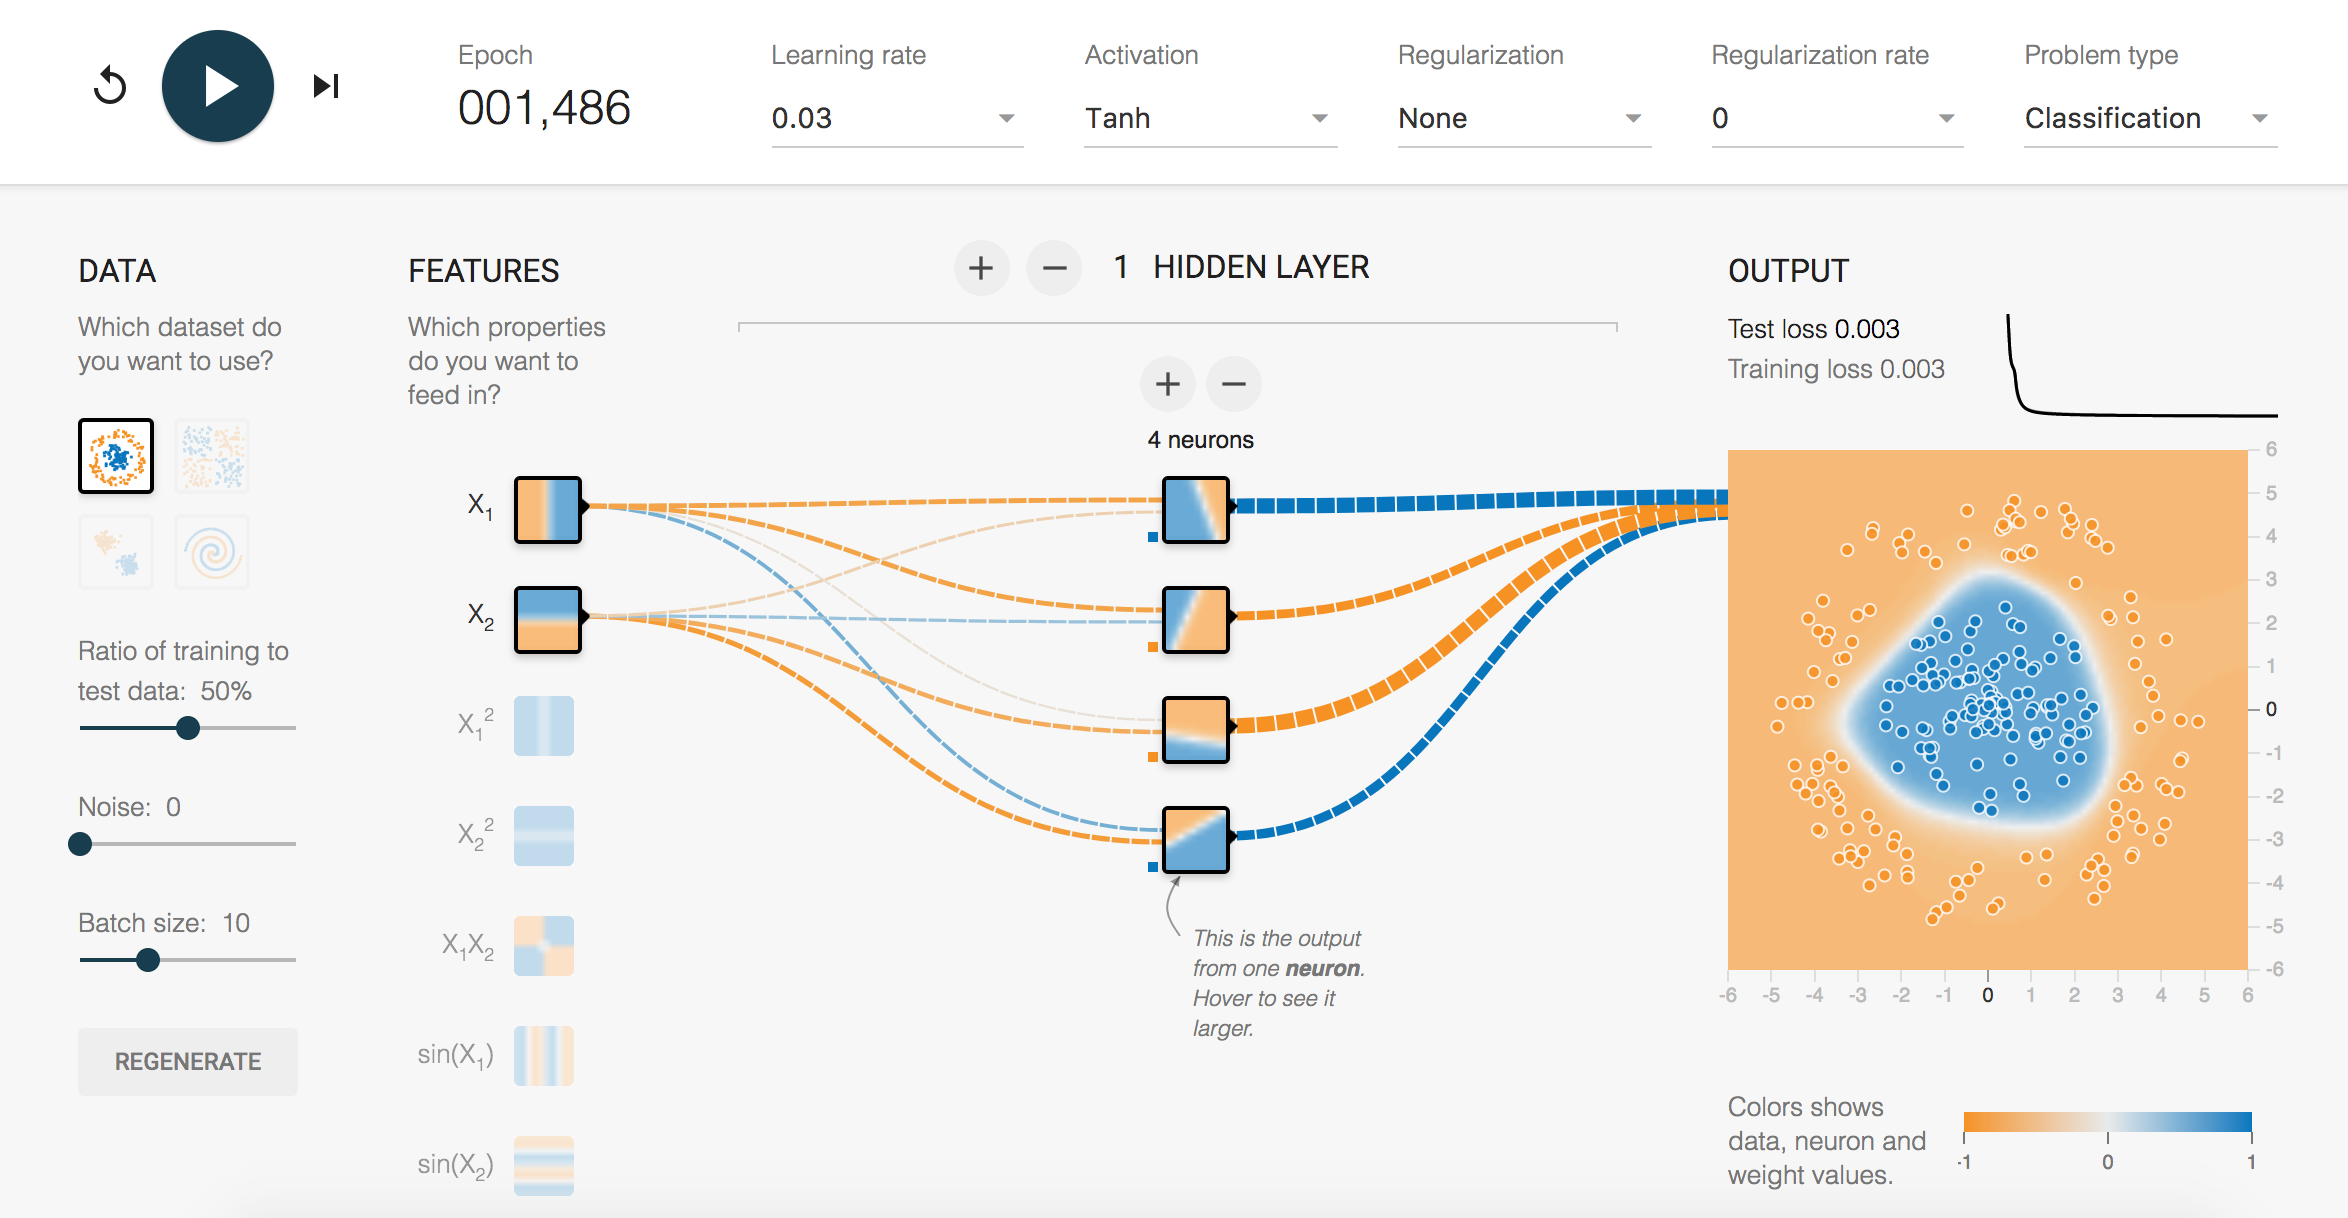
\includegraphics[width=0.87\textwidth,height=0.51\textheight,keepaspectratio]{images/lecture_4/tensorflow-playground.png}

		\href{https://playground.tensorflow.org/}{\textbf{playground.tensorflow.org}}
	\end{center}
	\small Change the number and width of the hidden layers. How do the learned representations and the decision boundary change?
\end{frame}


\subsection{Activation functions}

% Approved 2026-09-15: introduce sigmoid saturation and vanishing gradients
% in the forthcoming autodiff deck. Here, begin directly with ReLU.
\begin{frame}{The rectified linear unit (ReLU)}
	\begin{columns}[c,onlytextwidth]
		\begin{column}{0.55\textwidth}
			The \myalert{rectified linear unit} is defined as:
			\[
				{\color{darkcerulean}\phi(s)=\max(0,s)}.
			\]
			In words: negative inputs become zero, positive inputs pass through unchanged.
		\end{column}
		\begin{column}{0.41\textwidth}
			\centering
			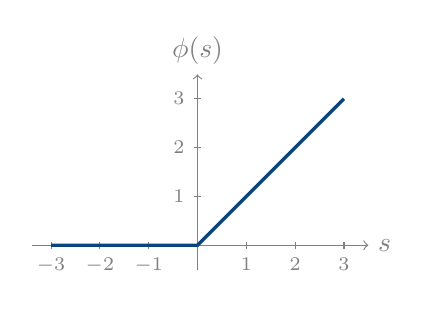
\begin{tikzpicture}[x=0.62cm,y=0.62cm]
				\draw[->,gray] (-3.4,0)--(3.5,0) node[right] {$s$};
				\draw[->,gray] (0,-0.5)--(0,3.5) node[above] {$\phi(s)$};
				\foreach \x in {-3,-2,-1,1,2,3}
				\draw[gray] (\x,0.07)--(\x,-0.07) node[below,font=\scriptsize] {$\x$};
				\foreach \y in {1,2,3}
				\draw[gray] (0.07,\y)--(-0.07,\y) node[left,font=\scriptsize] {$\y$};
				\draw[darkcerulean,very thick] (-3,0)--(0,0)--(3,3);
			\end{tikzpicture}
		\end{column}
	\end{columns}
	\vspace{1.2em}
	\small ReLU is a good default choice for MLPs: we will explain more in the automatic differentiation lecture, when we study how gradients propagate through the network.
\end{frame}


% Activation-section draft, 2026-09-15. Source mapping:
% "Variants of the ReLU (2)" + comparison -> smooth weighting + focused plots.
% LeakyReLU + "Trainable activation function" -> learning the negative slope.
% "Non-parametric AFs" -> basis expansion with KAF research connection.
% KAN -> corrected comparison of node activations and edge functions.
% Proposed omission for review: ELU/SELU catalogue entries.
% Trainable-Swish/GLU/Llama material deferred to parallel/multiplicative blocks.
% Prerequisites: scalar activations, affine maps, joint training (Basic definitions).
% g is a scalar weight; alpha is trained; psi_k are fixed basis functions.

\begin{frame}{ReLU as a gate}
	\small\setlength{\parskip}{5pt}\setlength{\abovedisplayskip}{8pt}\setlength{\belowdisplayskip}{8pt}
	\begin{columns}[c,onlytextwidth]
		\begin{column}{0.54\textwidth}
			ReLU can be interpreted as a multiplication of the input by an on/off gate:
			\[
				\operatorname{ReLU}(s)=s\,g(s),\qquad
				g(s)=\begin{cases}0 & s<0,\\1 & s\geq0.\end{cases}
			\]

			We can replace this hard decision with a \textbf{smooth weight} $g(s)$ between zero and one to obtain several interesting variants.
		\end{column}
		\begin{column}{0.43\textwidth}\centering\setlength{\parskip}{0pt}
			\textbf{Weight $g(s)$}\par
			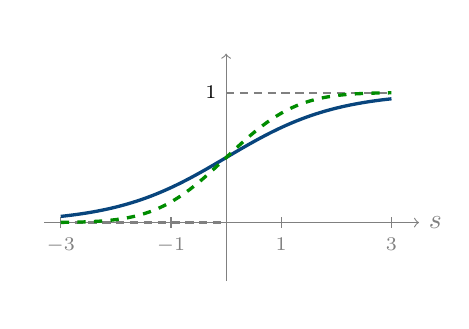
\begin{tikzpicture}[x=0.70cm,y=1.65cm]\path[use as bounding box] (-3.6,-0.6) rectangle (3.9,1.5);
				\draw[->,gray] (-3.3,0)--(3.5,0) node[right] {$s$};\draw[->,gray] (0,-0.45)--(0,1.3);\foreach \x in {-3,-1,1,3}\draw[gray] (\x,0.04)--(\x,-0.04) node[below,font=\scriptsize] {$\x$};\draw[gray,thick,densely dashed] (-3,0)--(0,0);\draw[gray,thick,densely dashed] (0,1)--(3,1);\node[left,font=\scriptsize] at (0,1) {$1$};\draw[darkcerulean,very thick] plot coordinates {(-3.0000,0.04743) (-2.9667,0.04895) (-2.9333,0.05053) (-2.9000,0.05215) (-2.8667,0.05383) (-2.8333,0.05555) (-2.8000,0.05732) (-2.7667,0.05915) (-2.7333,0.06103) (-2.7000,0.06297) (-2.6667,0.06497) (-2.6333,0.06702) (-2.6000,0.06914) (-2.5667,0.07131) (-2.5333,0.07355) (-2.5000,0.07586) (-2.4667,0.07823) (-2.4333,0.08067) (-2.4000,0.08317) (-2.3667,0.08575) (-2.3333,0.08840) (-2.3000,0.09112) (-2.2667,0.09392) (-2.2333,0.09680) (-2.2000,0.09975) (-2.1667,0.10278) (-2.1333,0.10590) (-2.1000,0.10910) (-2.0667,0.11238) (-2.0333,0.11575) (-2.0000,0.11920) (-1.9667,0.12275) (-1.9333,0.12638) (-1.9000,0.13011) (-1.8667,0.13393) (-1.8333,0.13784) (-1.8000,0.14185) (-1.7667,0.14596) (-1.7333,0.15016) (-1.7000,0.15447) (-1.6667,0.15887) (-1.6333,0.16337) (-1.6000,0.16798) (-1.5667,0.17269) (-1.5333,0.17751) (-1.5000,0.18243) (-1.4667,0.18745) (-1.4333,0.19258) (-1.4000,0.19782) (-1.3667,0.20316) (-1.3333,0.20861) (-1.3000,0.21417) (-1.2667,0.21983) (-1.2333,0.22560) (-1.2000,0.23148) (-1.1667,0.23746) (-1.1333,0.24355) (-1.1000,0.24974) (-1.0667,0.25604) (-1.0333,0.26244) (-1.0000,0.26894) (-0.9667,0.27555) (-0.9333,0.28225) (-0.9000,0.28905) (-0.8667,0.29595) (-0.8333,0.30294) (-0.8000,0.31003) (-0.7667,0.31720) (-0.7333,0.32446) (-0.7000,0.33181) (-0.6667,0.33924) (-0.6333,0.34676) (-0.6000,0.35434) (-0.5667,0.36201) (-0.5333,0.36974) (-0.5000,0.37754) (-0.4667,0.38541) (-0.4333,0.39333) (-0.4000,0.40131) (-0.3667,0.40935) (-0.3333,0.41743) (-0.3000,0.42556) (-0.2667,0.43373) (-0.2333,0.44193) (-0.2000,0.45017) (-0.1667,0.45843) (-0.1333,0.46672) (-0.1000,0.47502) (-0.0667,0.48334) (-0.0333,0.49167) (0.0000,0.50000) (0.0333,0.50833) (0.0667,0.51666) (0.1000,0.52498) (0.1333,0.53328) (0.1667,0.54157) (0.2000,0.54983) (0.2333,0.55807) (0.2667,0.56627) (0.3000,0.57444) (0.3333,0.58257) (0.3667,0.59065) (0.4000,0.59869) (0.4333,0.60667) (0.4667,0.61459) (0.5000,0.62246) (0.5333,0.63026) (0.5667,0.63799) (0.6000,0.64566) (0.6333,0.65324) (0.6667,0.66076) (0.7000,0.66819) (0.7333,0.67554) (0.7667,0.68280) (0.8000,0.68997) (0.8333,0.69706) (0.8667,0.70405) (0.9000,0.71095) (0.9333,0.71775) (0.9667,0.72445) (1.0000,0.73106) (1.0333,0.73756) (1.0667,0.74396) (1.1000,0.75026) (1.1333,0.75645) (1.1667,0.76254) (1.2000,0.76852) (1.2333,0.77440) (1.2667,0.78017) (1.3000,0.78583) (1.3333,0.79139) (1.3667,0.79684) (1.4000,0.80218) (1.4333,0.80742) (1.4667,0.81255) (1.5000,0.81757) (1.5333,0.82249) (1.5667,0.82731) (1.6000,0.83202) (1.6333,0.83663) (1.6667,0.84113) (1.7000,0.84553) (1.7333,0.84984) (1.7667,0.85404) (1.8000,0.85815) (1.8333,0.86216) (1.8667,0.86607) (1.9000,0.86989) (1.9333,0.87362) (1.9667,0.87725) (2.0000,0.88080) (2.0333,0.88425) (2.0667,0.88762) (2.1000,0.89090) (2.1333,0.89410) (2.1667,0.89722) (2.2000,0.90025) (2.2333,0.90320) (2.2667,0.90608) (2.3000,0.90888) (2.3333,0.91160) (2.3667,0.91425) (2.4000,0.91683) (2.4333,0.91933) (2.4667,0.92177) (2.5000,0.92414) (2.5333,0.92645) (2.5667,0.92869) (2.6000,0.93086) (2.6333,0.93298) (2.6667,0.93503) (2.7000,0.93703) (2.7333,0.93897) (2.7667,0.94085) (2.8000,0.94268) (2.8333,0.94445) (2.8667,0.94617) (2.9000,0.94785) (2.9333,0.94947) (2.9667,0.95105) (3.0000,0.95257)};\draw[darkgreen,very thick,dashed] plot coordinates {(-3.0000,0.00135) (-2.9667,0.00151) (-2.9333,0.00168) (-2.9000,0.00187) (-2.8667,0.00207) (-2.8333,0.00230) (-2.8000,0.00256) (-2.7667,0.00283) (-2.7333,0.00313) (-2.7000,0.00347) (-2.6667,0.00383) (-2.6333,0.00423) (-2.6000,0.00466) (-2.5667,0.00513) (-2.5333,0.00565) (-2.5000,0.00621) (-2.4667,0.00682) (-2.4333,0.00748) (-2.4000,0.00820) (-2.3667,0.00897) (-2.3333,0.00982) (-2.3000,0.01072) (-2.2667,0.01171) (-2.2333,0.01276) (-2.2000,0.01390) (-2.1667,0.01513) (-2.1333,0.01645) (-2.1000,0.01786) (-2.0667,0.01938) (-2.0333,0.02101) (-2.0000,0.02275) (-1.9667,0.02461) (-1.9333,0.02660) (-1.9000,0.02872) (-1.8667,0.03097) (-1.8333,0.03338) (-1.8000,0.03593) (-1.7667,0.03864) (-1.7333,0.04152) (-1.7000,0.04457) (-1.6667,0.04779) (-1.6333,0.05120) (-1.6000,0.05480) (-1.5667,0.05860) (-1.5333,0.06260) (-1.5000,0.06681) (-1.4667,0.07123) (-1.4333,0.07588) (-1.4000,0.08076) (-1.3667,0.08586) (-1.3333,0.09121) (-1.3000,0.09680) (-1.2667,0.10264) (-1.2333,0.10873) (-1.2000,0.11507) (-1.1667,0.12167) (-1.1333,0.12854) (-1.1000,0.13567) (-1.0667,0.14306) (-1.0333,0.15072) (-1.0000,0.15866) (-0.9667,0.16686) (-0.9333,0.17532) (-0.9000,0.18406) (-0.8667,0.19306) (-0.8333,0.20233) (-0.8000,0.21186) (-0.7667,0.22164) (-0.7333,0.23168) (-0.7000,0.24196) (-0.6667,0.25249) (-0.6333,0.26326) (-0.6000,0.27425) (-0.5667,0.28547) (-0.5333,0.29690) (-0.5000,0.30854) (-0.4667,0.32037) (-0.4333,0.33239) (-0.4000,0.34458) (-0.3667,0.35693) (-0.3333,0.36944) (-0.3000,0.38209) (-0.2667,0.39486) (-0.2333,0.40775) (-0.2000,0.42074) (-0.1667,0.43382) (-0.1333,0.44696) (-0.1000,0.46017) (-0.0667,0.47342) (-0.0333,0.48670) (0.0000,0.50000) (0.0333,0.51330) (0.0667,0.52658) (0.1000,0.53983) (0.1333,0.55304) (0.1667,0.56618) (0.2000,0.57926) (0.2333,0.59225) (0.2667,0.60514) (0.3000,0.61791) (0.3333,0.63056) (0.3667,0.64307) (0.4000,0.65542) (0.4333,0.66761) (0.4667,0.67963) (0.5000,0.69146) (0.5333,0.70310) (0.5667,0.71453) (0.6000,0.72575) (0.6333,0.73674) (0.6667,0.74751) (0.7000,0.75804) (0.7333,0.76832) (0.7667,0.77836) (0.8000,0.78814) (0.8333,0.79767) (0.8667,0.80694) (0.9000,0.81594) (0.9333,0.82468) (0.9667,0.83314) (1.0000,0.84134) (1.0333,0.84928) (1.0667,0.85694) (1.1000,0.86433) (1.1333,0.87146) (1.1667,0.87833) (1.2000,0.88493) (1.2333,0.89127) (1.2667,0.89736) (1.3000,0.90320) (1.3333,0.90879) (1.3667,0.91414) (1.4000,0.91924) (1.4333,0.92412) (1.4667,0.92877) (1.5000,0.93319) (1.5333,0.93740) (1.5667,0.94140) (1.6000,0.94520) (1.6333,0.94880) (1.6667,0.95221) (1.7000,0.95543) (1.7333,0.95848) (1.7667,0.96136) (1.8000,0.96407) (1.8333,0.96662) (1.8667,0.96903) (1.9000,0.97128) (1.9333,0.97340) (1.9667,0.97539) (2.0000,0.97725) (2.0333,0.97899) (2.0667,0.98062) (2.1000,0.98214) (2.1333,0.98355) (2.1667,0.98487) (2.2000,0.98610) (2.2333,0.98724) (2.2667,0.98829) (2.3000,0.98928) (2.3333,0.99018) (2.3667,0.99103) (2.4000,0.99180) (2.4333,0.99252) (2.4667,0.99318) (2.5000,0.99379) (2.5333,0.99435) (2.5667,0.99487) (2.6000,0.99534) (2.6333,0.99577) (2.6667,0.99617) (2.7000,0.99653) (2.7333,0.99687) (2.7667,0.99717) (2.8000,0.99744) (2.8333,0.99770) (2.8667,0.99793) (2.9000,0.99813) (2.9333,0.99832) (2.9667,0.99849) (3.0000,0.99865)};\end{tikzpicture}

			{\scriptsize\begin{tabular}{c}\color{drawgray}Dashed gray: hard gate\\\color{darkcerulean}Solid blue: sigmoid $\sigma(s)$\\\color{darkgreen}Dashed green: Gaussian CDF $\Phi(s)$\end{tabular}}
		\end{column}
	\end{columns}
\end{frame}

\begin{frame}{SiLU and GELU}
	\small\setlength{\parskip}{5pt}\setlength{\abovedisplayskip}{8pt}\setlength{\belowdisplayskip}{8pt}
	\begin{columns}[c,onlytextwidth]
		\begin{column}{0.54\textwidth}
			\textbf{SiLU} ({Sigmoid-weighted linear unit}):
			\[
				\operatorname{SiLU}(s)=s\,\sigma(s),\qquad
				\sigma(s)=\frac{1}{1+e^{-s}}.
			\]
			\vspace{0.5em}
			\textbf{GELU} ({Gaussian error linear unit}):
			\[
				\operatorname{GELU}(s)=s\,\Phi(s).
			\]
			{\small where $\Phi$ is the standard Gaussian cumulative distribution function.}
		\end{column}
		\begin{column}{0.43\textwidth}\centering\setlength{\parskip}{0pt}
			\textbf{Activation $s\,g(s)$}\par
			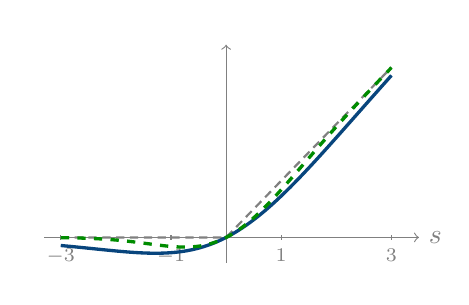
\begin{tikzpicture}[x=0.70cm,y=0.72cm]\path[use as bounding box] (-3.6,-0.7) rectangle (3.9,3.7);
				\draw[->,gray] (-3.3,0)--(3.5,0) node[right] {$s$};\draw[->,gray] (0,-0.45)--(0,3.4);\foreach \x in {-3,-1,1,3}\draw[gray] (\x,0.04)--(\x,-0.04) node[below,font=\scriptsize] {$\x$};\draw[gray,thick,densely dashed] (-3,0)--(0,0)--(3,3);\draw[darkcerulean,very thick] plot coordinates {(-3.0000,-0.14228) (-2.9667,-0.14523) (-2.9333,-0.14822) (-2.9000,-0.15125) (-2.8667,-0.15430) (-2.8333,-0.15739) (-2.8000,-0.16051) (-2.7667,-0.16365) (-2.7333,-0.16683) (-2.7000,-0.17003) (-2.6667,-0.17325) (-2.6333,-0.17650) (-2.6000,-0.17976) (-2.5667,-0.18304) (-2.5333,-0.18634) (-2.5000,-0.18965) (-2.4667,-0.19296) (-2.4333,-0.19629) (-2.4000,-0.19961) (-2.3667,-0.20294) (-2.3333,-0.20627) (-2.3000,-0.20958) (-2.2667,-0.21289) (-2.2333,-0.21618) (-2.2000,-0.21945) (-2.1667,-0.22270) (-2.1333,-0.22592) (-2.1000,-0.22910) (-2.0667,-0.23225) (-2.0333,-0.23535) (-2.0000,-0.23841) (-1.9667,-0.24140) (-1.9333,-0.24434) (-1.9000,-0.24721) (-1.8667,-0.25000) (-1.8333,-0.25271) (-1.8000,-0.25533) (-1.7667,-0.25786) (-1.7333,-0.26028) (-1.7000,-0.26259) (-1.6667,-0.26478) (-1.6333,-0.26684) (-1.6000,-0.26877) (-1.5667,-0.27055) (-1.5333,-0.27218) (-1.5000,-0.27364) (-1.4667,-0.27493) (-1.4333,-0.27603) (-1.4000,-0.27694) (-1.3667,-0.27765) (-1.3333,-0.27814) (-1.3000,-0.27841) (-1.2667,-0.27845) (-1.2333,-0.27824) (-1.2000,-0.27777) (-1.1667,-0.27703) (-1.1333,-0.27602) (-1.1000,-0.27471) (-1.0667,-0.27311) (-1.0333,-0.27119) (-1.0000,-0.26894) (-0.9667,-0.26636) (-0.9333,-0.26343) (-0.9000,-0.26015) (-0.8667,-0.25649) (-0.8333,-0.25245) (-0.8000,-0.24802) (-0.7667,-0.24319) (-0.7333,-0.23794) (-0.7000,-0.23227) (-0.6667,-0.22616) (-0.6333,-0.21961) (-0.6000,-0.21261) (-0.5667,-0.20514) (-0.5333,-0.19719) (-0.5000,-0.18877) (-0.4667,-0.17986) (-0.4333,-0.17044) (-0.4000,-0.16052) (-0.3667,-0.15009) (-0.3333,-0.13914) (-0.3000,-0.12767) (-0.2667,-0.11566) (-0.2333,-0.10312) (-0.2000,-0.09003) (-0.1667,-0.07640) (-0.1333,-0.06223) (-0.1000,-0.04750) (-0.0667,-0.03222) (-0.0333,-0.01639) (0.0000,0.00000) (0.0333,0.01694) (0.0667,0.03444) (0.1000,0.05250) (0.1333,0.07110) (0.1667,0.09026) (0.2000,0.10997) (0.2333,0.13022) (0.2667,0.15101) (0.3000,0.17233) (0.3333,0.19419) (0.3667,0.21657) (0.4000,0.23948) (0.4333,0.26289) (0.4667,0.28681) (0.5000,0.31123) (0.5333,0.33614) (0.5667,0.36153) (0.6000,0.38739) (0.6333,0.41372) (0.6667,0.44050) (0.7000,0.46773) (0.7333,0.49539) (0.7667,0.52348) (0.8000,0.55198) (0.8333,0.58088) (0.8667,0.61018) (0.9000,0.63985) (0.9333,0.66990) (0.9667,0.70031) (1.0000,0.73106) (1.0333,0.76215) (1.0667,0.79356) (1.1000,0.82529) (1.1333,0.85731) (1.1667,0.88963) (1.2000,0.92223) (1.2333,0.95510) (1.2667,0.98822) (1.3000,1.02159) (1.3333,1.05519) (1.3667,1.08902) (1.4000,1.12306) (1.4333,1.15730) (1.4667,1.19174) (1.5000,1.22636) (1.5333,1.26116) (1.5667,1.29612) (1.6000,1.33123) (1.6333,1.36649) (1.6667,1.40188) (1.7000,1.43741) (1.7333,1.47305) (1.7667,1.50881) (1.8000,1.54467) (1.8333,1.58062) (1.8667,1.61667) (1.9000,1.65279) (1.9333,1.68899) (1.9667,1.72526) (2.0000,1.76159) (2.0333,1.79798) (2.0667,1.83442) (2.1000,1.87090) (2.1333,1.90742) (2.1667,1.94397) (2.2000,1.98055) (2.2333,2.01715) (2.2667,2.05378) (2.3000,2.09042) (2.3333,2.12707) (2.3667,2.16372) (2.4000,2.20039) (2.4333,2.23705) (2.4667,2.27370) (2.5000,2.31035) (2.5333,2.34700) (2.5667,2.38363) (2.6000,2.42024) (2.6333,2.45684) (2.6667,2.49342) (2.7000,2.52997) (2.7333,2.56650) (2.7667,2.60301) (2.8000,2.63949) (2.8333,2.67594) (2.8667,2.71237) (2.9000,2.74875) (2.9333,2.78511) (2.9667,2.82143) (3.0000,2.85772)};\draw[darkgreen,very thick,dashed] plot coordinates {(-3.0000,-0.00405) (-2.9667,-0.00447) (-2.9333,-0.00492) (-2.9000,-0.00541) (-2.8667,-0.00595) (-2.8333,-0.00653) (-2.8000,-0.00715) (-2.7667,-0.00783) (-2.7333,-0.00857) (-2.7000,-0.00936) (-2.6667,-0.01021) (-2.6333,-0.01113) (-2.6000,-0.01212) (-2.5667,-0.01318) (-2.5333,-0.01431) (-2.5000,-0.01552) (-2.4667,-0.01682) (-2.4333,-0.01820) (-2.4000,-0.01967) (-2.3667,-0.02124) (-2.3333,-0.02290) (-2.3000,-0.02467) (-2.2667,-0.02653) (-2.2333,-0.02851) (-2.2000,-0.03059) (-2.1667,-0.03278) (-2.1333,-0.03509) (-2.1000,-0.03752) (-2.0667,-0.04006) (-2.0333,-0.04272) (-2.0000,-0.04550) (-1.9667,-0.04840) (-1.9333,-0.05142) (-1.9000,-0.05456) (-1.8667,-0.05782) (-1.8333,-0.06119) (-1.8000,-0.06467) (-1.7667,-0.06827) (-1.7333,-0.07196) (-1.7000,-0.07576) (-1.6667,-0.07965) (-1.6333,-0.08363) (-1.6000,-0.08768) (-1.5667,-0.09180) (-1.5333,-0.09598) (-1.5000,-0.10021) (-1.4667,-0.10448) (-1.4333,-0.10876) (-1.4000,-0.11306) (-1.3667,-0.11735) (-1.3333,-0.12161) (-1.3000,-0.12584) (-1.2667,-0.13001) (-1.2333,-0.13410) (-1.2000,-0.13808) (-1.1667,-0.14195) (-1.1333,-0.14568) (-1.1000,-0.14923) (-1.0667,-0.15260) (-1.0333,-0.15575) (-1.0000,-0.15866) (-0.9667,-0.16129) (-0.9333,-0.16364) (-0.9000,-0.16565) (-0.8667,-0.16732) (-0.8333,-0.16861) (-0.8000,-0.16948) (-0.7667,-0.16992) (-0.7333,-0.16990) (-0.7000,-0.16937) (-0.6667,-0.16833) (-0.6333,-0.16673) (-0.6000,-0.16455) (-0.5667,-0.16177) (-0.5333,-0.15835) (-0.5000,-0.15427) (-0.4667,-0.14951) (-0.4333,-0.14403) (-0.4000,-0.13783) (-0.3667,-0.13088) (-0.3333,-0.12315) (-0.3000,-0.11463) (-0.2667,-0.10530) (-0.2333,-0.09514) (-0.2000,-0.08415) (-0.1667,-0.07230) (-0.1333,-0.05960) (-0.1000,-0.04602) (-0.0667,-0.03156) (-0.0333,-0.01622) (0.0000,0.00000) (0.0333,0.01711) (0.0667,0.03511) (0.1000,0.05398) (0.1333,0.07374) (0.1667,0.09436) (0.2000,0.11585) (0.2333,0.13819) (0.2667,0.16137) (0.3000,0.18537) (0.3333,0.21019) (0.3667,0.23579) (0.4000,0.26217) (0.4333,0.28930) (0.4667,0.31716) (0.5000,0.34573) (0.5333,0.37499) (0.5667,0.40490) (0.6000,0.43545) (0.6333,0.46660) (0.6667,0.49834) (0.7000,0.53063) (0.7333,0.56344) (0.7667,0.59674) (0.8000,0.63052) (0.8333,0.66473) (0.8667,0.69935) (0.9000,0.73435) (0.9333,0.76970) (0.9667,0.80537) (1.0000,0.84134) (1.0333,0.87759) (1.0667,0.91407) (1.1000,0.95077) (1.1333,0.98766) (1.1667,1.02472) (1.2000,1.06192) (1.2333,1.09924) (1.2667,1.13666) (1.3000,1.17416) (1.3333,1.21172) (1.3667,1.24932) (1.4000,1.28694) (1.4333,1.32457) (1.4667,1.36219) (1.5000,1.39979) (1.5333,1.43735) (1.5667,1.47487) (1.6000,1.51232) (1.6333,1.54971) (1.6667,1.58702) (1.7000,1.62424) (1.7333,1.66137) (1.7667,1.69840) (1.8000,1.73533) (1.8333,1.77214) (1.8667,1.80885) (1.9000,1.84544) (1.9333,1.88191) (1.9667,1.91827) (2.0000,1.95450) (2.0333,1.99061) (2.0667,2.02661) (2.1000,2.06248) (2.1333,2.09824) (2.1667,2.13388) (2.2000,2.16941) (2.2333,2.20483) (2.2667,2.24013) (2.3000,2.27533) (2.3333,2.31043) (2.3667,2.34543) (2.4000,2.38033) (2.4333,2.41513) (2.4667,2.44985) (2.5000,2.48448) (2.5333,2.51902) (2.5667,2.55349) (2.6000,2.58788) (2.6333,2.62220) (2.6667,2.65645) (2.7000,2.69064) (2.7333,2.72476) (2.7667,2.75883) (2.8000,2.79285) (2.8333,2.82681) (2.8667,2.86072) (2.9000,2.89459) (2.9333,2.92841) (2.9667,2.96220) (3.0000,2.99595)};\end{tikzpicture}

			{\scriptsize\begin{tabular}{c}\color{drawgray}Dashed gray: ReLU\\\color{darkcerulean}Solid blue: SiLU\\\color{darkgreen}Dashed green: GELU\end{tabular}}
		\end{column}
	\end{columns}
	\vspace{0.6em}
	{\tiny\color{drawgray}\href{https://arxiv.org/abs/1702.03118}{Elfwing et al. (2017)}; \href{https://arxiv.org/abs/1606.08415}{Hendrycks and Gimpel (2016)}.}
\end{frame}

\begin{frame}{Learning the negative slope}
	\small\setlength{\abovedisplayskip}{4pt}\setlength{\belowdisplayskip}{4pt}\setlength{\parskip}{3pt}
	Instead of fixing the whole activation, we can let training adjust its shape.
	\[
		\phi_{\alpha}(s)=\begin{cases}s & s\geq0,\\ \alpha s & s<0.\end{cases}
	\]
	\begin{columns}[T,onlytextwidth]
		\begin{column}{0.49\textwidth}
			\begin{tcolorbox}[nndsblue,height=0.28\textheight]
				\textbf{LeakyReLU}\\[0.4em]
				\small Fix a small negative-side slope, e.g., $\alpha=0.01$.
			\end{tcolorbox}
		\end{column}
		\begin{column}{0.49\textwidth}
			\begin{tcolorbox}[nndsgreen,height=0.28\textheight]
				\textbf{Parametric ReLU (PReLU)}\\[0.4em]
				\small Learn $\alpha$ jointly with the weights and biases.
			\end{tcolorbox}
		\end{column}
	\end{columns}
	\small For PReLU, $\alpha$ is part of $\boldsymbol{\theta}$. It can be shared or learned separately for different units.
	\vfill
	{\scriptsize\color{drawgray}\href{https://arxiv.org/abs/1502.01852}{He et al. (2015), Delving Deep into Rectifiers}.}
\end{frame}

\begin{frame}{Learning the activation shape}
	\small\setlength{\abovedisplayskip}{4pt}\setlength{\belowdisplayskip}{4pt}\setlength{\parskip}{3pt}
	Learn a more flexible shape using fixed \textbf{basis functions}:
	\[
		{\color{darkcerulean}\phi(s)=\sum_{k=1}^{K}\alpha_k\psi_k(s)}.
	\]
	The coefficients $\alpha_k$ are trained jointly with the network.
	\begin{tcolorbox}[nndsblue]
		\small\setlength{\abovedisplayskip}{4pt}\setlength{\belowdisplayskip}{4pt}\setlength{\parskip}{3pt}\textbf{Kernel activation functions (KAFs)}
		\[
			\psi_k(s)=\kappa(s,d_k),\qquad
			\kappa(s,d_k)=\exp\!\bigl(-\gamma(s-d_k)^2\bigr).
		\]
		Example: Gaussian bumps with fixed centers $d_k$ and width parameter $\gamma>0$.
	\end{tcolorbox}
	\textbf{Non-parametric}: a flexible basis expansion, still implemented with finitely many parameters. Splines are another option.
	\vfill
	{\scriptsize\color{drawgray}\href{https://arxiv.org/abs/1707.04035}{Scardapane et al. (2019), Kafnets}.}
\end{frame}

\begin{frame}{Kolmogorov--Arnold networks}
	\small\setlength{\abovedisplayskip}{4pt}\setlength{\belowdisplayskip}{4pt}\setlength{\parskip}{3pt}
	We can also change where the learned scalar functions act:
	\begin{columns}[T,onlytextwidth]
		\begin{column}{0.49\textwidth}
			\begin{tcolorbox}[nndsblue,height=0.40\textheight]
				\small\setlength{\abovedisplayskip}{4pt}\setlength{\belowdisplayskip}{4pt}\setlength{\parskip}{3pt}\textbf{MLP with learned activations}
				\[h_i=\phi_i\!\left(\textstyle\sum_j W_{ij}x_j+b_i\right).\]
				Mix inputs, then transform each unit.
			\end{tcolorbox}
		\end{column}
		\begin{column}{0.49\textwidth}
			\begin{tcolorbox}[nndsgreen,height=0.40\textheight]
				\small\setlength{\abovedisplayskip}{4pt}\setlength{\belowdisplayskip}{4pt}\setlength{\parskip}{3pt}\textbf{KAN layer}
				\[h_i=\textstyle\sum_jW_{ij}\phi_{ij}(x_j).\]
				Transform each connection, then sum.
			\end{tcolorbox}
		\end{column}
	\end{columns}
	A KAF learns an activation at a unit, while a KAN learns functions on connections. Flexibility, however, comes with additional parameters and computation, making them less efficient that (equivalently deep) ReLU-based models.
	\vfill
	{\scriptsize\color{drawgray}\href{https://arxiv.org/abs/2404.19756}{Liu et al. (2024), KAN: Kolmogorov--Arnold Networks}.}
\end{frame}

\subsection{Combining layers beyond the basic MLP}


% Diagram styles used only by the six closing slides.
\tikzset{
	nnblock/.style={
			draw=drawblue, fill=drawblue_l!25!white, rounded corners=2pt,
			minimum width=1.25cm, minimum height=0.65cm,
			inner sep=5pt, font=\small
		},
	nnother/.style={nnblock, draw=drawgreen, fill=drawgreen_l!25!white},
	nnmerge/.style={
			circle, draw=drawgray, fill=white,
			minimum size=0.55cm, inner sep=1pt, font=\small
		},
	nnedge/.style={->, thick, draw=drawgray}
}

\begin{frame}{Combining branches}
	\small
	\setlength{\parskip}{3pt}
	\setlength{\abovedisplayskip}{5pt}
	\setlength{\belowdisplayskip}{5pt}
	Two blocks can also process the same input in parallel. Given
	$\vc{u}=f(\vc{x})$ and $\vc{v}=g(\vc{x})$, we can combine their outputs in different ways:

	\begin{columns}[c,onlytextwidth]
		\begin{column}{0.56\textwidth}
			\begin{itemize}
				\setlength{\itemsep}{3pt}
				\item \textbf{Concatenation}, $[\vc{u};\vc{v}]$, preserves both
				      feature vectors and adds their widths.
				\item \textbf{Addition}, $\vc{u}+\vc{v}$, combines matching
				      coordinates and requires equal shapes.
				\item Choosing the identity for one branch gives a
				      \textbf{residual connection}: $\vc{y}=\vc{x}+f(\vc{x})$.
			\end{itemize}
		\end{column}
		\begin{column}{0.41\textwidth}
			\centering
			\begin{tikzpicture}[x=1cm,y=1cm]
			\node (x) at (0,0) {$\vc{x}$};
\coordinate (split) at (0.65,0);

			\node[nnblock] (f) at (2,0.75) {$f$};
\node[nnother] (g) at (2,-0.75) {$\mathrm{id}$};

			\node[nnmerge] (m) at (4,0) {$+$};
\node (y) at (5.1,0) {$\vc{y}$};

			\draw[thick,drawgray] (x)--(split);
\fill[drawgray] (split) circle (1.5pt);

			\draw[nnedge] (split)|-(f);
\draw[nnedge] (split)|-(g);

			\draw[nnedge] (f.east)--(3.25,0.75)-|(m.north);
\draw[nnedge] (g.east)--(3.25,-0.75)-|(m.south);
\draw[nnedge] (m)--(y);

		\end{tikzpicture}

		\end{column}
	\end{columns}
	\vfill
	{\tiny\color{drawgray}
		Concatenation example: \href{https://arxiv.org/abs/1608.06993}{DenseNet (2017)};
		residual networks: \href{https://arxiv.org/abs/1512.03385}{He et al. (2016)}.\par}
\end{frame}

\begin{frame}{Input-dependent branch weights}
	\small
	\setlength{\parskip}{3pt}
	\setlength{\abovedisplayskip}{5pt}
	\setlength{\belowdisplayskip}{5pt}
	Instead of adding branches with fixed coefficients, we can learn weights
	that depend on the input.

	\begin{columns}[T,onlytextwidth]
		\begin{column}{0.49\textwidth}
			\begin{tcolorbox}[nndsblue,height=5.05cm,boxsep=2pt,left=5pt,right=5pt,top=5pt,bottom=5pt]
				\footnotesize\RaggedRight
				\setlength{\parskip}{3pt}
				\setlength{\abovedisplayskip}{5pt}
				\setlength{\belowdisplayskip}{5pt}
				\textbf{Highway connections}
				\begin{align*}
					\vc{t} & = \sigma(\vc{W}_t\vc{x}+\vc{b}_t), \\
					\vc{y} & = \vc{t}\odot f(\vc{x})
					+(\vc{1}-\vc{t})\odot\vc{x}.
				\end{align*}
				Each gate coordinate lies in $[0,1]$ and controls how much of the
				input is carried forward. Similar gates appear in recurrent models;
				$\odot$ denotes elementwise multiplication.
			\end{tcolorbox}
		\end{column}
		\begin{column}{0.49\textwidth}
			\begin{tcolorbox}[nndsgreen,height=5.05cm,boxsep=2pt,left=5pt,right=5pt,top=5pt,bottom=5pt]
				\footnotesize\RaggedRight
				\setlength{\parskip}{3pt}
				\setlength{\abovedisplayskip}{5pt}
				\setlength{\belowdisplayskip}{5pt}
				\textbf{Mixtures of experts (MoEs)}
				\[
					\vc{y}=\sum_{e=1}^{E}a_e(\vc{x})f_e(\vc{x}).
				\]
				A router weights the outputs of several experts with the same
				output shape. Sparse MoEs, used in language models, save computation
				by evaluating only the selected experts.
			\end{tcolorbox}
		\end{column}
	\end{columns}

	\vfill
	{\tiny\color{drawgray}
		\href{https://arxiv.org/abs/1505.00387}{Srivastava et al., Highway Networks (2015)};
		\href{https://arxiv.org/abs/1701.06538}{Shazeer et al., Sparsely-Gated MoEs (2017)}.\par}
\end{frame}

\begin{frame}{Multiplicative blocks: GLU and SwiGLU}
	\small
	\setlength{\parskip}{3pt}
	\setlength{\abovedisplayskip}{5pt}
	\setlength{\belowdisplayskip}{5pt}
	We can also multiply two branch outputs elementwise. In a GLU block,
	one projection determines how the other is weighted:

	\begin{center}
		\begin{tikzpicture}
			\node (x) at (0,0) {$\vc{x}$};
\node[nnblock] (u) at (1.8,0.65) {$\vc{W}_u$};
\node[nnother] (g) at (1.8,-0.65) {$\vc{W}_g$};
\node[nnother] (phi) at (3.5,-0.65) {$\phi$};
\node[nnmerge] (m) at (5,0) {$\odot$};
\node[nnblock] (o) at (6.5,0) {$\vc{W}_o$};
\node (y) at (7.9,0) {$\vc{y}$};

			\draw[nnedge] (x)|-(u);
\draw[nnedge] (x)|-(g);
\draw[nnedge] (g)--(phi);
\draw[nnedge] (u.east)--(5,0.65)--(m.north);
\draw[nnedge] (phi.east)-|(m.south);
\draw[nnedge] (m)--(o);
\draw[nnedge] (o)--(y);

		\end{tikzpicture}

	\end{center}
	\[
		\vc{y}=\vc{W}_o\left[(\vc{W}_u\vc{x})\odot\phi(\vc{W}_g\vc{x})\right].
	\]
	With $\phi=\sigma$ we obtain a \textbf{GLU}, whose gate lies in $[0,1]$.
	Replacing it with SiLU gives \textbf{SwiGLU}, used in Llama: its multiplier
	can also be negative or exceed one.

		{\footnotesize For $\vc{x}\in\mathbb{R}^{D}$,
			$\vc{W}_u,\vc{W}_g\in\mathbb{R}^{M\times D}$ and $\vc{W}_o\in\mathbb{R}^{D\times M}$.
			Biases are omitted.\par}
	\vfill
	{\tiny\color{drawgray}
		\href{https://arxiv.org/abs/2002.05202}{Shazeer (2020)};
		\href{https://arxiv.org/abs/2302.13971}{Touvron et al., LLaMA (2023)}.\par}
\end{frame}

\begin{frame}{Sharing parameters and looping a block}
	\small
	\setlength{\parskip}{3pt}
	\setlength{\abovedisplayskip}{5pt}
	\setlength{\belowdisplayskip}{5pt}
	A stack can use different parameters at each layer, or repeatedly apply
	the same block. The latter gives a \textbf{looped model}:\vspace{0.5em}

	\begin{columns}[c,onlytextwidth]
		\begin{column}{0.60\textwidth}
			\textbf{Separate parameters}
			\begin{center}
				\input{images/lecture_4/untied.tex}
			\end{center}
			\textbf{Shared parameters}
			\begin{center}
				\begin{tikzpicture}[x=0.83cm]\node (x) at (0,0) {$\vc{h}^{(0)}$};
\node[nnblock] (b0) at (1.6,0) {$f_{\boldsymbol{\theta}}$};
\node[nnblock] (b1) at (3.6,0) {$f_{\boldsymbol{\theta}}$};
\node[nnblock] (b2) at (5.6,0) {$f_{\boldsymbol{\theta}}$};
\node (y) at (7.3,0) {$\vc{h}^{(3)}$};
\draw[nnedge] (x)--(b0);
\draw[nnedge] (b0)--(b1);
\draw[nnedge] (b1)--(b2);
\draw[nnedge] (b2)--(y);
\end{tikzpicture}

			\end{center}
		\end{column}
		\begin{column}{0.38\textwidth}
			\centering
			\begin{tikzpicture}
			\node (x) at (0,0) {$\vc{h}^{(0)}$};
\node[nnblock,minimum width=1.8cm] (f) at (2.1,0) {$f_{\boldsymbol{\theta}}$};
\node (y) at (4.3,0) {$\vc{h}^{(L)}$};

			\draw[nnedge] (x)--(f);
\draw[nnedge] (f)--(y);
\draw[nnedge] (3.2,0)--(3.2,1.05)--node[above,font=\scriptsize] {repeat $L$ times} (1,1.05)--(1,0);

		\end{tikzpicture}

		\end{column}
	\end{columns}

	The shared block computes $\vc{h}^{(\ell+1)}=f_{\boldsymbol{\theta}}(\vc{h}^{(\ell)})$,
	with matching input and output shapes. For a block with $P$ parameters,
	sharing reduces the count from $LP$ to $P$, but still requires $L$ evaluations.
	\vfill
	{\tiny\color{drawgray}
		The unrolled example shows three applications.
		\href{https://arxiv.org/abs/1807.03819}{Dehghani et al., Universal Transformers (2019)}.\par}
\end{frame}

\begin{frame}{Recurrence over a sequence}
	\small
	\setlength{\parskip}{3pt}
	\setlength{\abovedisplayskip}{5pt}
	\setlength{\belowdisplayskip}{5pt}
	If we supply a new input at each application, the shared block becomes
	a \textbf{recurrent model}:
	\[
		\vc{h}_t=f_{\boldsymbol{\theta}}(\vc{h}_{t-1},\vc{x}_t).
	\]
	\begin{center}
		\begin{tikzpicture}
			\node (h0) at (0,0) {$\vc{h}_0$};

			
\foreach \i in {1,2,3}{\node[nnblock] (b\i) at (2*\i,0) {$f_{\boldsymbol{\theta}}$};
\node (x\i) at (2*\i,0.95) {$\vc{x}_{\i}$};
\draw[nnedge] (x\i)--(b\i);
}
			\node (h3) at (8,0) {$\vc{h}_3$};
\draw[nnedge] (h0)--(b1);
\draw[nnedge] (b1)--node[below,font=\scriptsize] {$\vc{h}_1$}(b2);
\draw[nnedge] (b2)--node[below,font=\scriptsize] {$\vc{h}_2$}(b3);
\draw[nnedge] (b3)--(h3);

		\end{tikzpicture}

	\end{center}

	The hidden state carries information from earlier inputs, while the same
	parameters are used throughout the sequence. The model can therefore process sequences of different lengths.

	Unlike a loop over depth, this recurrence advances through the input sequence
	at each step.
\end{frame}

\begin{frame}{Shared MLPs on structured data}
	\small
	\setlength{\parskip}{3pt}
	\setlength{\abovedisplayskip}{5pt}
	\setlength{\belowdisplayskip}{5pt}
	An MLP can process each position of a sequence $\vc{X}\sim(T,D)$ independently,
	using the same parameters:
	\begin{columns}[c,onlytextwidth]
		\begin{column}{0.51\textwidth}
			\[
				\idx{\vc{Y}}{t,:}=f_{\boldsymbol{\theta}}(\idx{\vc{X}}{t,:}).
			\]
			This mixes features within a position, but does not exchange
			information between positions.
		\end{column}
		\begin{column}{0.46\textwidth}
			\centering
			\begin{tikzpicture}[x=0.8cm,y=0.8cm]
			
\foreach \i in {1,2,3}{\pgfmathtruncatemacro{\pos}{\i-1}\node (x\i) at (2.7*\i,1.05) {$\idx{\vc{X}}{\pos,:}$};
\node[nnblock] (f\i) at (2.7*\i,0) {$f_{\boldsymbol{\theta}}$};
\node (y\i) at (2.7*\i,-1.05) {$\idx{\vc{Y}}{\pos,:}$};
\draw[nnedge] (x\i)--(f\i);
\draw[nnedge] (f\i)--(y\i);
}
		\end{tikzpicture}

		\end{column}
	\end{columns}

	The same idea applies to image pixels or patch vectors. Flattening the
	whole image instead allows global mixing, but ties the weights to a fixed layout.

	Transformers use these \textbf{positionwise MLPs} alongside attention.
	Communication between positions requires another operation, such as
	convolution over neighborhoods, attention, or a recurrent state.
\end{frame}

\end{document}
